\documentclass[notitlepage]{article}
\usepackage[utf8]{inputenc} 
\usepackage{geometry} 		
\usepackage{chngcntr}
\usepackage{amsmath} 			
\usepackage{amssymb}			
\usepackage{mathtools}		
\usepackage{comment} 			
\usepackage{mdframed}			
\usepackage{xcolor}				
\usepackage{fancyhdr}			
\usepackage{listings}			
\usepackage{color}				
\usepackage{tikz}	
\usepackage{tasks}			
\usepackage{exsheets}		
\usepackage{array}			
\usepackage{empheq}
\usepackage{caption}
\usepackage{pdfpages}
\usepackage{tabularx}

\geometry{ 						%Format titlepage (interrupted by newgeometry)
	a4paper,
	total={170mm,257mm}%,
	%left=0mm,
	%top=0mm,
}

%START DEFINE YOUR VARIABLES HERE

\newcommand{\documentName}{Software Design Specification}
\newcommand{\projectName}{Label Refinement by Behavioral Similarity}

%END DEFINE YOUR VARIABLES HERE

\title{%
	\documentName\text{ } \\
  \large \projectName\text{ } \\
  }

\author{
	\large \underline{Document owners:}\\ 
	Bianka Bakullari\\
	\texttt{}
	Christopher Beine\\
	\texttt{}
	Nicole Ventsch\\
	\texttt{}
	Juan Garza\\
	\texttt{}
}

\date{\small{Last edited: \today}}

\pagestyle{fancy}
\fancyhf{}
\rhead{}
\lhead{\documentName\space-\space\projectName}

\makeatletter					%Prefix to add ToC to titlepage
\newcommand*{\toccontents}{\@starttoc{toc}}
\renewcommand*\contentsname{}
\makeatother
                  

\begin{document}

\begin{titlepage}
\clearpage\maketitle			%Clear title page
\thispagestyle{fancy}
\tableofcontents
\end{titlepage}

\rfoot{\thepage}				%Start printing page-numbers, after title page.

\newgeometry{ 					%Default page formatting on-going #1
	total={170mm,257mm},
	left=20mm,
	top=25mm,
    bottom=30mm					%Causes warning
}

\begin{flushleft}				%Default page formatting on-going #2


\section{Introduction}
\subsection{System Overview}
\subsection{Design Map}
\subsection{Supporting Materials}
\subsection{Definitions and Acronyms}

\section{Design Considerations}
\subsection{Assumptions}
\subsection{Constraints}
\subsection{System Environment}
\subsection{Design Methodology}
\subsection{Risks and Volatile Areas}

\section{Architecture}
\subsection{Overview}
\subsection{Rationale}
\subsection{Component Details}

\section{High Level Design}
\subsection{Conceptual View}

\section{Low Level Design}
\subsection{Module 1}
\subsection{Module 2}
%.....

\section{User Interface Design}
\subsection{Application Control}
\subsection{Screen 1}

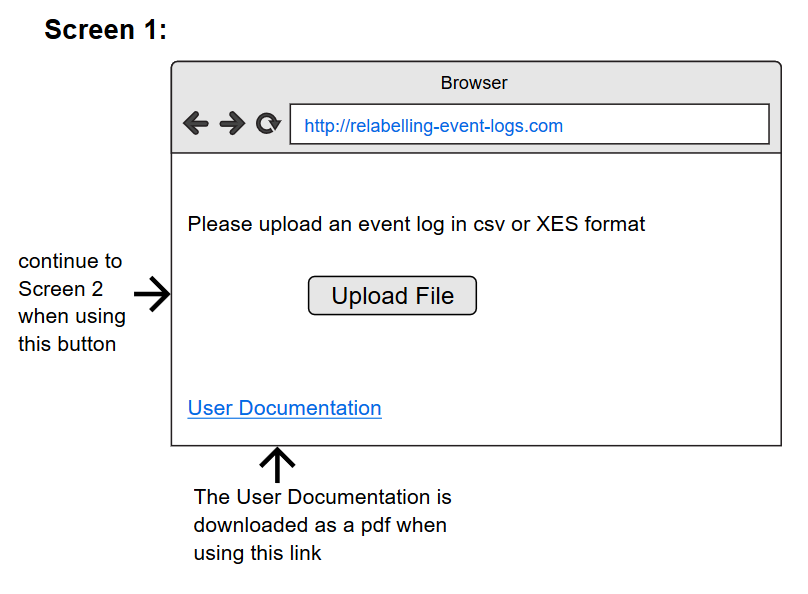
\includegraphics[scale=0.8]{InterfaceMockup1.png}


The first screen visible to the user will show a description saying that an event log in csv of XES format should be uploaded. Moreover, a button "Upload File" is visible. By using this button, the user will continue to Screen 2. At the end of the page, there will be a link called "User Documentation". By clicking on this link, the User Documentation will be downloaded in pdf format.
\subsection{Screen 2}

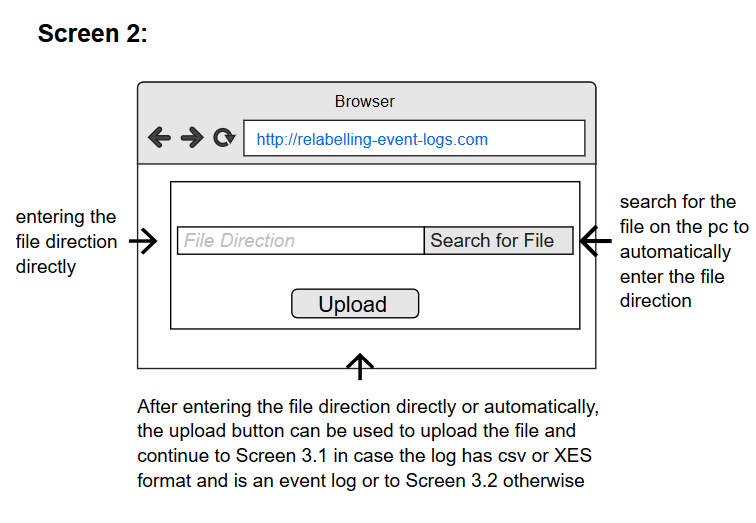
\includegraphics[scale=0.8]{InterfaceMockup2.png}

In the second screen visible to the user, the user can enter the file direction of the event log he wants to upload. He can either directly type in the direction into the "File Direction" field or use the "search for File" button to search for a file on his pc, so that the direction will automatically be filled in after selecting a file.

After using one of this alternatives, he can use the "Upload" button to upload the file with the given directory. In case this file is an event log, i.e., the data contains at least the attributes "id", "time stamp" and "activity name", and has either csv or XES format, the user will continue to Screen 3.1. If one of these conditions is not satisfied, he will continue to Screen 3.2. 

\subsection{Screen 3}

Depending on whether the file the user uploaded meets the constraints, either Screen 3.1 or Screen 3.2 will be shown.

\subsubsection{Screen 3.1}
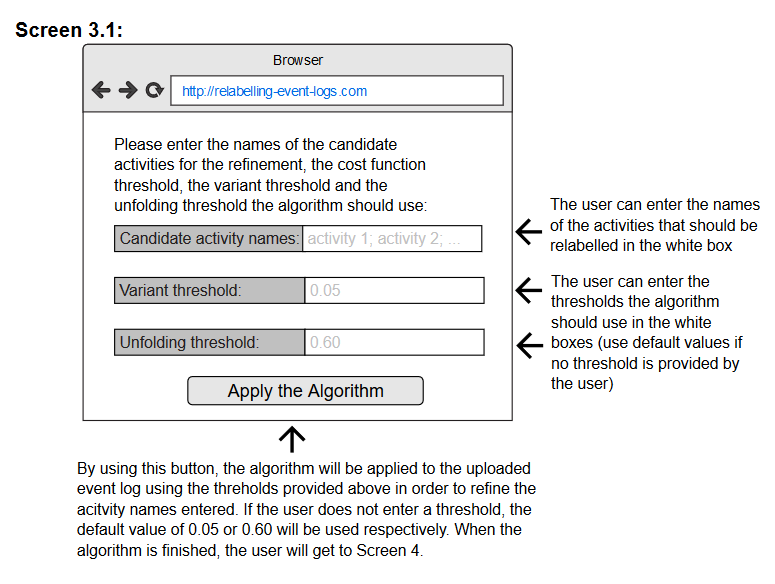
\includegraphics[scale=0.8]{InterfaceMockup3-1.png}

This screen appears if the file uploaded by the user meets the requirements. In this screen, the user can set the thresholds for the algorithm, i.e., the variant and the unfolding threshold. He can enter these in the corresponding white boxes. If he does not enter the thresholds, the default values of 0.05 and 0.60 will be used respectively. Using the button "Apply the Algorithm", the web service will start applying the algorithm using the provided thresholds. After the algorithm is finished, the user will get to Screen 4.

\subsubsection{Screen 3.2}
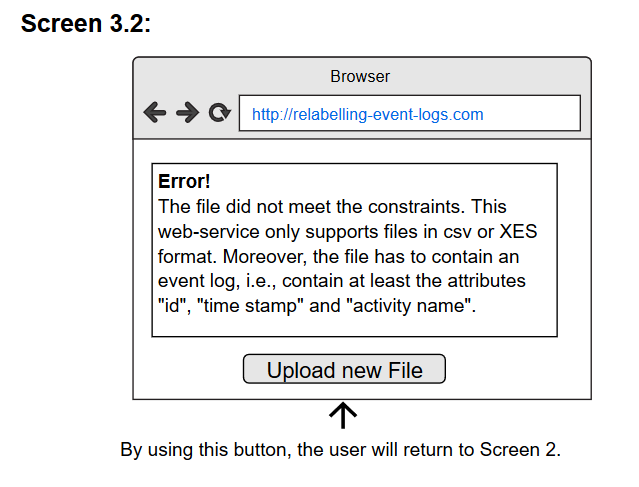
\includegraphics[scale=0.8]{InterfaceMockup3-2.png}

This screen appears if the upload was not successful because the file did not meet the assumptions. If the file does not have the right format, the user can click on the button "Upload new File" to return to Screen 2 and upload a file that meets the constraints.


\subsection{Screen 4}
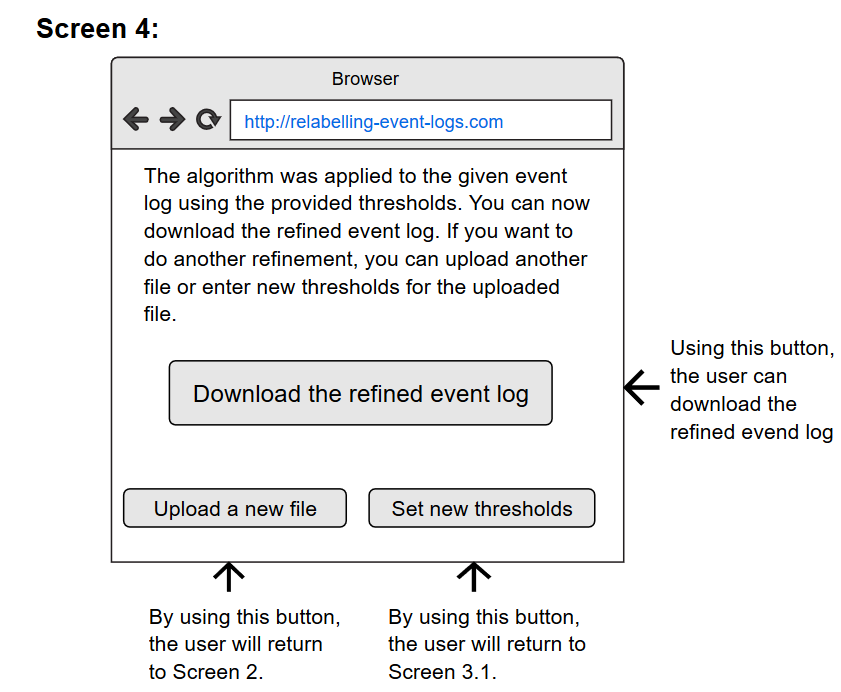
\includegraphics[scale=0.8]{InterfaceMockup4.png}

This Screen will be shown after finishing the algorithm. The user can now download the refined log using the corresponding button. After this step, the user is done and can exit the page, but if he also wants to apply the algorithm to another event log or to the same event log using different thresholds, he can use the corresponding buttons and will be redirected to Screen 2 or Screen 3.1 respectively.


%\newpage
%\bibliographystyle{plain}
%\bibliography{references}  




%\addcontentsline{toc}{chapter}{\textbf{References}}
\end{flushleft}
%\bibliography{uw-ethesis}
% Tip 5: You can create multiple .bib files to organize your references. 
% Just list them all in the \bibliogaphy command, separated by commas (no spaces).

% The following statement causes the specified references to be added to the bibliography% even if they were not 
% cited in the text. The asterisk is a wildcard that causes all entries in the bibliographic database to be included (optional).


\begin{thebibliography}{5}
\bibitem{paper}
Lu, Xixi, et al. "Handling duplicated tasks in process discovery by refining event labels." International Conference on Business Process Management. Springer, Cham, 2016.




\end{thebibliography}










\end{document}
